\hypertarget{appendix}{%
\section*{Appendix}\label{appendix}}
\addcontentsline{toc}{section}{Appendix}

\tableofcontents
\listoffigures

\newpage

\begin{multicols}{2}

\hypertarget{introduction}{%
\section{Introduction}\label{introduction}}

\textbf{YASP optionchain visualiser} is a collection of multiple
technologies: \textbf{Python} as the programming language, \textbf{Bash}
as a scripting language, \textbf{JSON} as a database, \textbf{Flask} as
a software-based server, \textbf{Raspberry Pi} as hardware and
\textbf{Arch Linux}\footnote{arch linux is used as it provides arch user
  repository which hosts a lot of commandline tools used in this project}
as operating system and setup environment .

Using web-scraping we extract data from NSE \footnote{National Stock
  Exchange www.nseindia.com} which gets saved in database (as json file)
then using matplotlib in first varient and dash(component in plotly
{[}\^{}plotty{]}) we generate static pngs and interactive graphs.

\hypertarget{mechanism}{%
\subsection{Mechanism}\label{mechanism}}

Both \textbf{varients}\footnote{see sec.~\ref{sec:varients}} of this
project scrape \textbf{NSE}\footnote{National Stock Exchange
  www.nseindia.com} to collect relevant data about user provieded stocks
or all the public stocks listed on the exchange.

After this is done, the collected json data is add to \emph{data}
subdirectory and named as \emph{stockname}-fno.json, this collected json
data is used to generate png graphs and present interactive dash using
plotly , served through a flask web server.This process is completly
done on a Raspberry Pi 4, hence can be used to achive a headless server
which does automated run of this script at fixed intervals 24x7.

\hypertarget{propose-work}{%
\section{Propose work}\label{propose-work}}

\hypertarget{probability-by-normal-distribution}{%
\subsection{Probability by normal
distribution}\label{probability-by-normal-distribution}}

Implied volatility is \emph{not} directly observable, so it needs to be
solved using the five other inputs of the Black-Scholes model, which
are:

\begin{itemize}
\tightlist
\item
  The market price of the option.
\item
  The underlying stock price.
\item
  The strike price.
\item
  The time to expiration.
\item
  The risk-free interest rate.
\end{itemize}

\hypertarget{market-price}{%
\subsubsection{Market Price}\label{market-price}}

The \textbf{market} \textbf{price} is the current price at which an
asset or service can be bought or sold. The market price of an asset or
service is determined by the forces of supply and demand. The price at
which quantity supplied equals quantity demanded is the market price.

Shocks to either the supply or the demand for a good or service can
cause the market price for a good or service to change. A
\textbf{supply} \textbf{shock} is an unexpected event that suddenly
changes the supply of a good or service. A demand shock is a sudden
event that increases or decreases the demand for a good or service. Some
examples of supply shock are interest rate cuts, tax cuts, government
stimulus, terrorist attacks, natural disasters, and stock market
crashes. Some examples of demand shock include a steep rise in oil and
gas prices or other commodities, political turmoil, natural disasters,
and breakthroughs in production technology.

\hypertarget{strike-price}{%
\subsubsection{Strike Price}\label{strike-price}}

A \textbf{strike} \textbf{price} is the set price at which a derivative
contract can be bought or sold when it is exercised. For call options,
the strike price is where the security can be bought by the option
holder; for put options, the strike price is the price at which the
security can be sold.

Strike prices are used in derivatives (mainly options) trading.
Derivatives are financial products whose value is based (derived) on the
underlying asset, usually another financial instrument. The strike price
is a key variable of call and put options. For example, the buyer of a
call option would have the right, but not the obligation, to buy the
underlying security in the future at the specified strike price.

\end{multicols}

\hypertarget{black-scholes}{%
\subsection{Black-Scholes}\label{black-scholes}}

Implied volatility is calculated by taking the market price of the
option, entering it into the \textbf{Black-Scholes} \textbf{formula},
and back-solving for the value of the volatility. But there are various
approaches to calculating implied volatility. One simple approach is to
use an iterative search, or trial and error, to find the value of
implied volatility. Iv calculation done by nse

\begin{quote}
Call IV :: call implied volatility (given by nse) put IV :: put option
implied volatility (given by nse) Days of expiry :: expiryDate ( today )
\end{quote}

\begin{quote}
Strike value win probability =
\end{quote}

\begin{quote}
NORMSDIST(LN(STRIKEPRICE/VALUE)/CALLIV*SQRT(DAYSTOEXPIRATION/365))
\end{quote}

\begin{quote}
NORMSDIST = (0.5*pi)\textsuperscript{2} * e\textsuperscript{(-(z²)/2)}
\end{quote}

\begin{Shaded}
\begin{Highlighting}[numbers=left,,]
  \ControlFlowTok{for}\NormalTok{ i }\KeywordTok{in}\NormalTok{ label:}
   \CommentTok{\#STRIKE\textless{}VALUE WIN PROB =\textgreater{} NORMSDIST(LN(STRIKEPRICE/VALUE)/CALLIV*SQRT(DAYSTOEXPIRATION/365))}
   \CommentTok{\#normsdist = (1/2pi)\^{}2 * e\^{}({-}(z\^{}2)/2)}
    \ControlFlowTok{if}\NormalTok{ i }\OperatorTok{\textless{}}\NormalTok{ value }\KeywordTok{and}\NormalTok{ i }\OperatorTok{\textgreater{}} \DecValTok{0}\NormalTok{:}
      \ControlFlowTok{try}\NormalTok{:}
\NormalTok{          normsdist }\OperatorTok{=}\NormalTok{ math.log(i}\OperatorTok{/}\NormalTok{underlyingValue) }\OperatorTok{/} \OperatorTok{\textbackslash{}}
\NormalTok{              ((iv\_call}\OperatorTok{/}\DecValTok{100}\NormalTok{)}\OperatorTok{*}\NormalTok{math.sqrt(daysexpiry}\OperatorTok{/}\DecValTok{365}\NormalTok{))}
\NormalTok{          result }\OperatorTok{=}\NormalTok{ integrate.quad(}\KeywordTok{lambda}\NormalTok{ q: (}
\NormalTok{              (}\DecValTok{1}\OperatorTok{/}\NormalTok{math.sqrt(}\DecValTok{2} \OperatorTok{*}\NormalTok{ math.pi))}\OperatorTok{*}\NormalTok{((math.e)}\OperatorTok{**}\NormalTok{(q}\OperatorTok{**}\DecValTok{2}\OperatorTok{/{-}}\FloatTok{2.0}\NormalTok{))), }\OperatorTok{{-}}\NormalTok{np.inf, normsdist)}
\NormalTok{          prob.append(}\DecValTok{100} \OperatorTok{{-}}\NormalTok{ result[}\DecValTok{0}\NormalTok{]}\OperatorTok{*}\DecValTok{100}\NormalTok{)}
        \ControlFlowTok{except}\NormalTok{:}
\NormalTok{            prob.append(}\DecValTok{0}\NormalTok{)}
    \ControlFlowTok{elif}\NormalTok{ i }\OperatorTok{\textgreater{}}\NormalTok{ value }\KeywordTok{and}\NormalTok{ i }\OperatorTok{\textgreater{}} \DecValTok{0}\NormalTok{:}
      \ControlFlowTok{try}\NormalTok{:}
\NormalTok{          normsdist }\OperatorTok{=}\NormalTok{ math.log(i}\OperatorTok{/}\NormalTok{underlyingValue) }\OperatorTok{/} \OperatorTok{\textbackslash{}}
\NormalTok{              ((iv\_put}\OperatorTok{/}\DecValTok{100}\NormalTok{)}\OperatorTok{*}\NormalTok{math.sqrt(daysexpiry}\OperatorTok{/}\DecValTok{365}\NormalTok{))}
\NormalTok{          result }\OperatorTok{=}\NormalTok{ integrate.quad(}\KeywordTok{lambda}\NormalTok{ q: (}
\NormalTok{              (}\DecValTok{1}\OperatorTok{/}\NormalTok{math.sqrt(}\DecValTok{2} \OperatorTok{*}\NormalTok{ math.pi))}\OperatorTok{*}\NormalTok{((math.e)}\OperatorTok{**}\NormalTok{(q}\OperatorTok{**}\DecValTok{2}\OperatorTok{/{-}}\FloatTok{2.0}\NormalTok{))), }\OperatorTok{{-}}\NormalTok{np.inf, normsdist)}
\NormalTok{          prob.append(result[}\DecValTok{0}\NormalTok{]}\OperatorTok{*}\DecValTok{100}\NormalTok{)}
      \ControlFlowTok{except}\NormalTok{:}
\NormalTok{          prob.append(}\DecValTok{0}\NormalTok{)}
    \ControlFlowTok{else}\NormalTok{:}
\NormalTok{        prob.append(}\DecValTok{0}\NormalTok{)}
\end{Highlighting}
\end{Shaded}

\begin{center}\rule{0.5\linewidth}{0.5pt}\end{center}

\hypertarget{components-in-black-scholes-formula}{%
\subsubsection{Components in Black-Scholes
formula}\label{components-in-black-scholes-formula}}

Calculation of theoretical base price of contracts as per Black--Scholes
formula: The options price for a Call option shall be computed as
follows:

\begin{verbatim}
 C = S * N (d1) – X * e^(-rt)^\* N (d2)
 and the price for a Put option is :
 P = X * e^(-rt)^\* N (-d2) – S * N (-d1)
 where :
 d1 = ln (S / X) + (r + s ^ 2 / 2) * t
 s * vt
 d2 = ln (S / X) + (r – s 2 / 2) * t
 s * vt = d1 - s * vt
 
 C = price of a Call option
 P = price of a Put option
 S = price of the underlying asset
 X = Strike price of the option
 r = rate of interest (Rate of interest shall be the relevant MIBOR rate for the day)
 t = time to expiration
 s = volatility 

 N represents standard normal distribution with mean = 0 and standard deviation = 1, 
 ln represents the natural logarithm of a number. 
 Natural logarithms are based on the constant e (2.71828182845904)
\end{verbatim}

\hypertarget{sec:varients}{%
\subsection{Different varients of the project}\label{sec:varients}}

\begin{multicols}{2}

\hypertarget{user-input-based}{%
\subsubsection{User input based}\label{user-input-based}}

This varient primarily relies on user to decide stock about which he/she
has to scrape information. Using the run \footnote{script used to
  install fzf and other dependencies like jq} script provided in the
repository user call the fzf \footnote{fuzzy finding prompt writtern in
  Go} prompt. In the fzf \footnote{fuzzy finding prompt writtern in Go}
prompt user is supposed to write name of the stock they want to search,
the search usses fuzzy algorithm \footnote{https://en.wikipedia.org/wiki/Approximate\_string\_matching}
, hence if we write \emph{SBI} in the search prompt, \textbf{SBIN} ,
\textbf{SBILIFE} , \textbf{SBICARD} gets displayed as results ; then
user can press tab to select the symbol \footnote{https://en.wikipedia.org/wiki/Ticker\_symbol}
on the promt and press it again to select the enxt prompt or search for
other symbol to add the array that will be fed to python script to start
the scrape.

\hypertarget{server-based-flask}{%
\subsubsection{Server based (Flask)}\label{server-based-flask}}

This varient runs bye just typing \textbf{python3 optionchain.py} in the
bash terminal. Goal of this varient is to run headleass\footnote{https://en.wikipedia.org/wiki/Headless\_computer}
on Raspberry Pi 4. A flask server is initiated which uses dash frontend
provieded by plotly\footnote{https://plotly.com/dash/} to show the user
interactive graphs generated using collected data . Six graphs are
produced for each ticker symbol chosen in the top menu by the user. See
figure \ref{mylabel}.

\end{multicols}

\begin{figure}
\centering
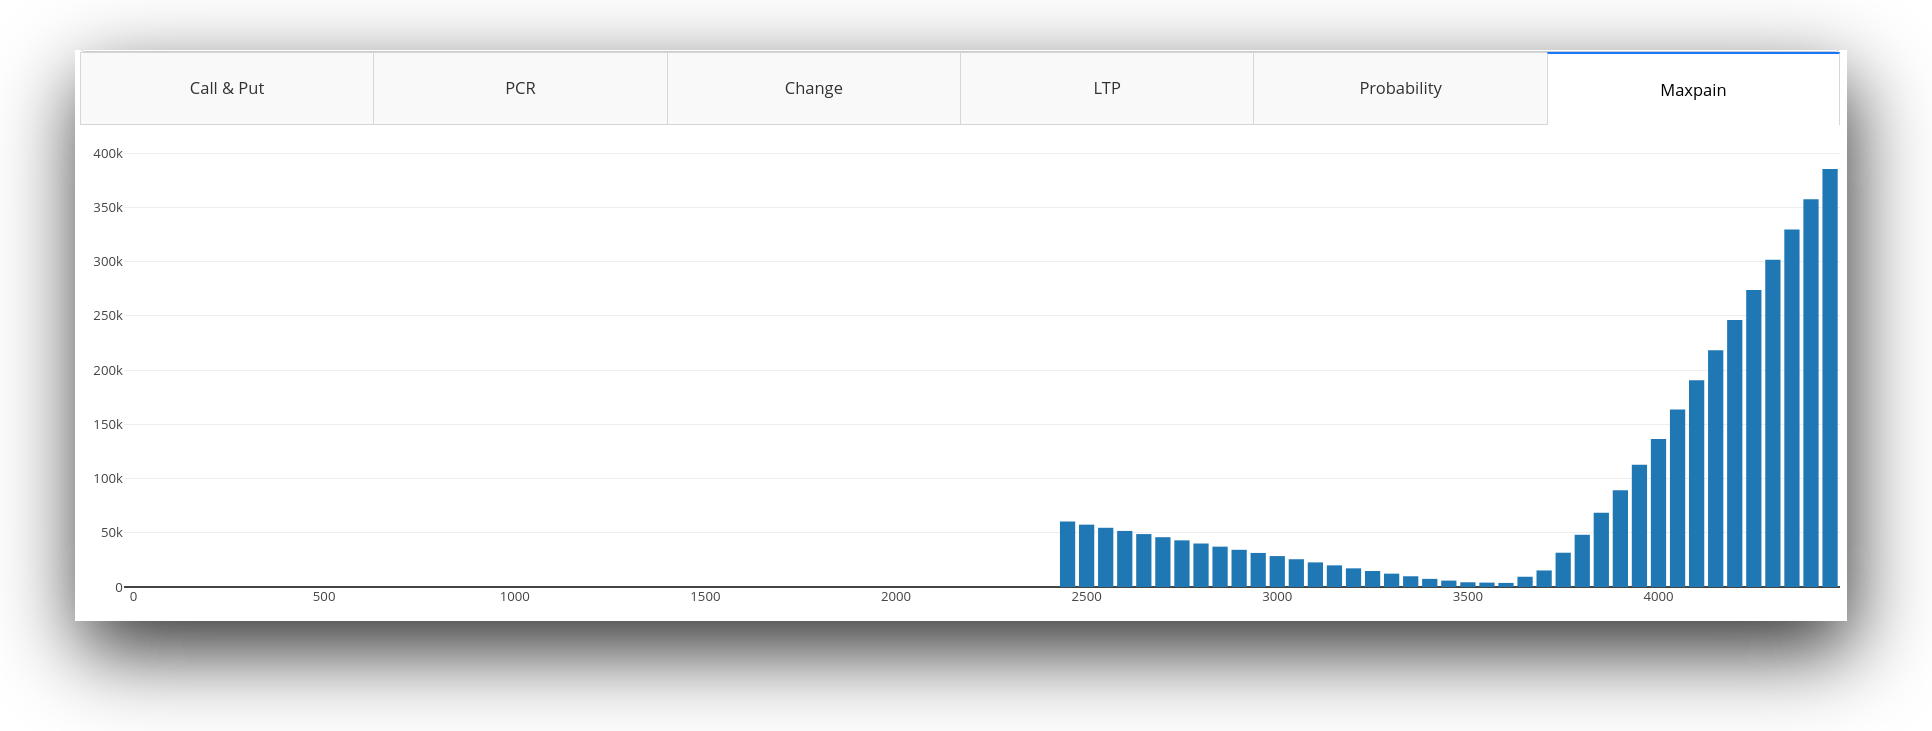
\includegraphics{main.png}
\caption{Generated Graph \label{mylabel}}
\end{figure}

\newpage

\hypertarget{generated-graphs-and-results}{%
\section{Generated Graphs and
Results}\label{generated-graphs-and-results}}

\begin{multicols}{2}

\hypertarget{call}{%
\subsection{Call}\label{call}}

\begin{itemize}
\tightlist
\item
  A call is an option contract giving the owner the right, but not the
  obligation, to buy a specified amount of an underlying security at a
  specified price within a specified time.
\item
  The specified price is known as the strike price and the specified
  time during which a sale is made is its expiration or time to
  maturity.
\item
  You pay a fee to purchase a call option, called the premium; this
  per-share charge is the maximum you can lose on a call option.
\item
  Call options may be purchased for speculation or sold for income
  purposes or for tax management.
\item
  Call options may also be combined for use in spread or combination
  strategies.
\end{itemize}

\begin{figure}
\centering
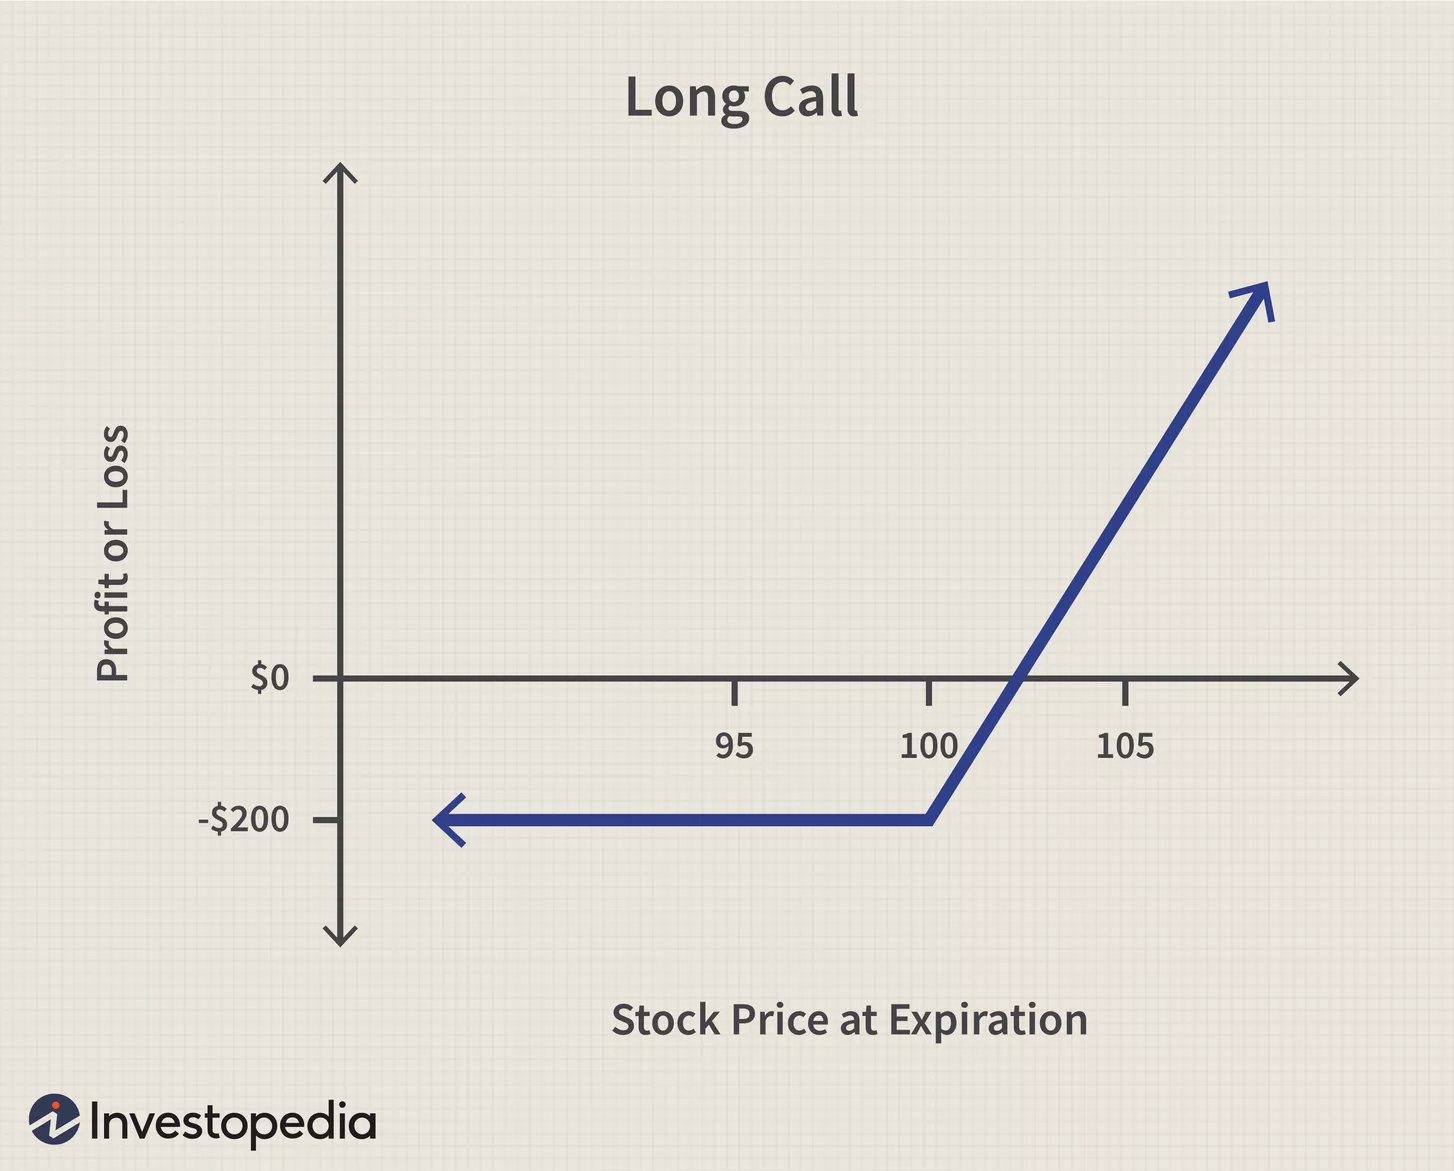
\includegraphics{call.png}
\caption{Image by Sabrina Jiang © Investopedia}
\end{figure}

\hypertarget{put}{%
\subsection{Put}\label{put}}

\begin{itemize}
\tightlist
\item
  Put options give holders of the option the right, but not the
  obligation, to sell a specified amount of an underlying security at a
  specified price within a specified time frame.
\item
  Put options are available on a wide range of assets, including stocks,
  indexes, commodities, and currencies.
\item
  Put option prices are impacted by changes in the price of the
  underlying asset, the option strike price, time decay, interest rates,
  and volatility.
\item
  Put options increase in value as the underlying asset falls in price,
  as volatility of the underlying asset price increases, and as interest
  rates decline.
\item
  Put options lose value as the underlying asset increases in price, as
  volatility of the underlying asset price decreases, as interest rates
  rise, and as the time to expiration nears.
\end{itemize}

\begin{figure}
\centering
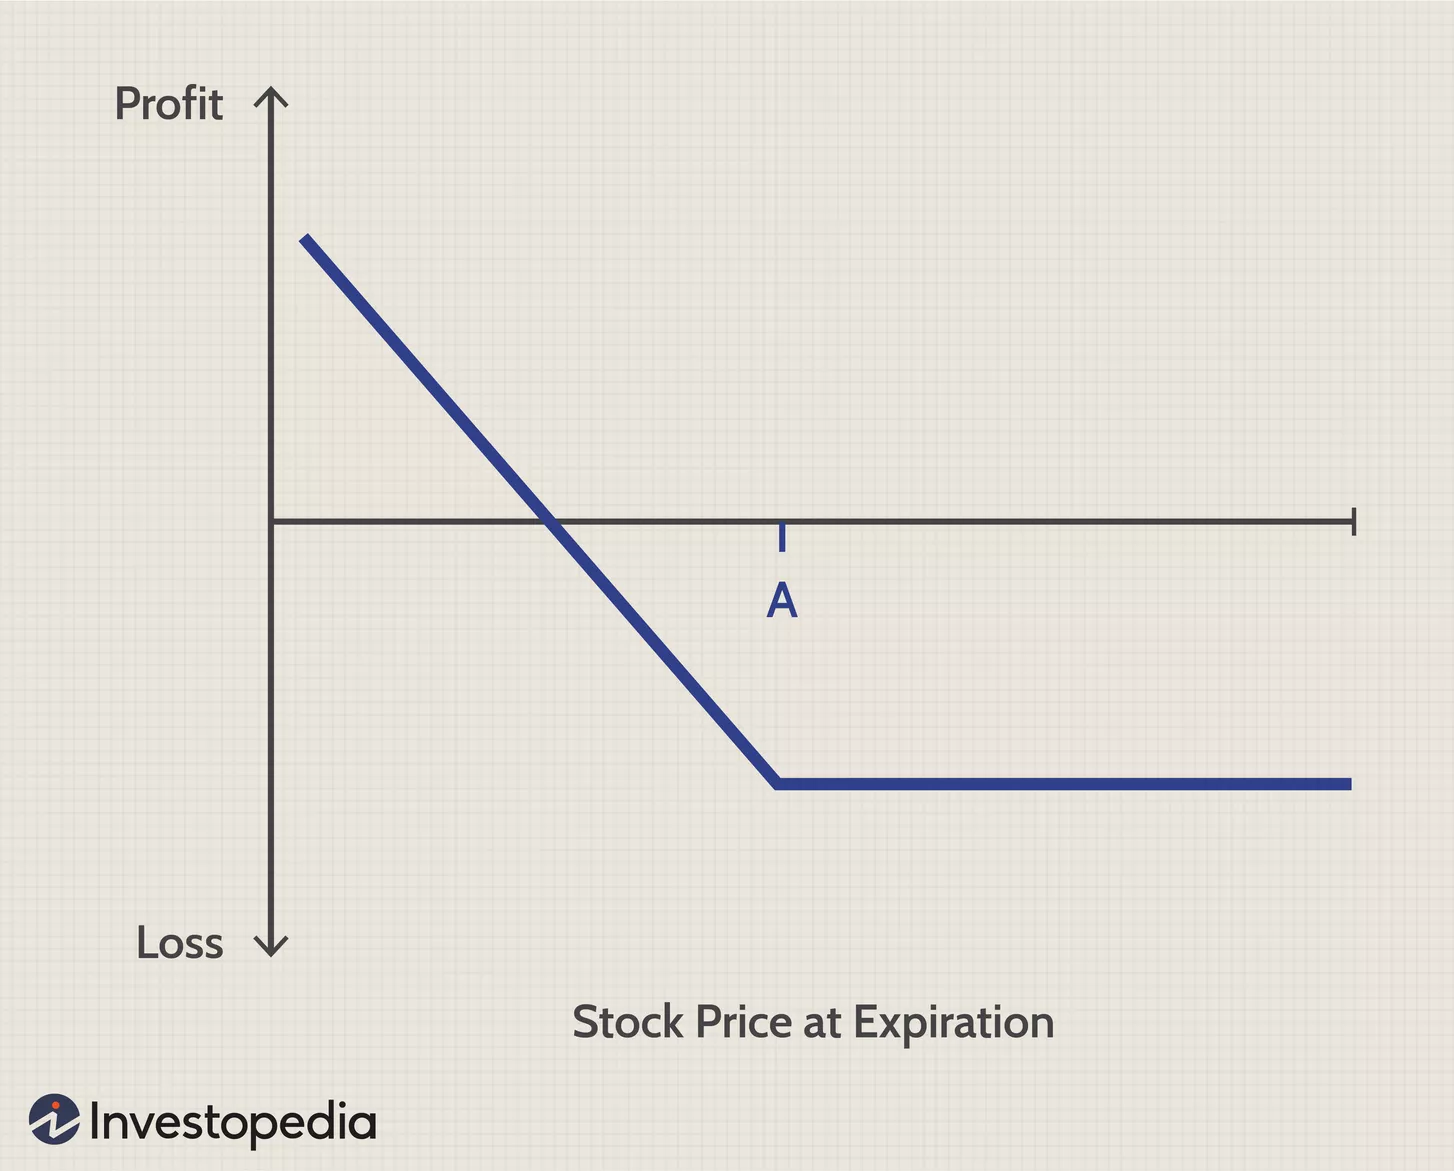
\includegraphics{put.png}
\caption{Image by Sabrina Jiang © Investopedia}
\end{figure}

\hypertarget{pcr}{%
\subsection{PCR}\label{pcr}}

The put-call ratio is a measurement that is widely used by investors to
gauge the overall mood of a market.

A ``put'' or put option is a right to sell an asset at a predetermined
price. A ``call'' or call option is a right to buy an asset at a
predetermined price. If traders are buying more puts than calls, it
signals a rise in bearish sentiment.

\end{multicols}

If they are buying more calls than puts, it suggests that they see a
bull market ahead\footnote{https://www.investopedia.com/ask/answers/06/putcallratio.asp}.

\begin{figure}
\centering
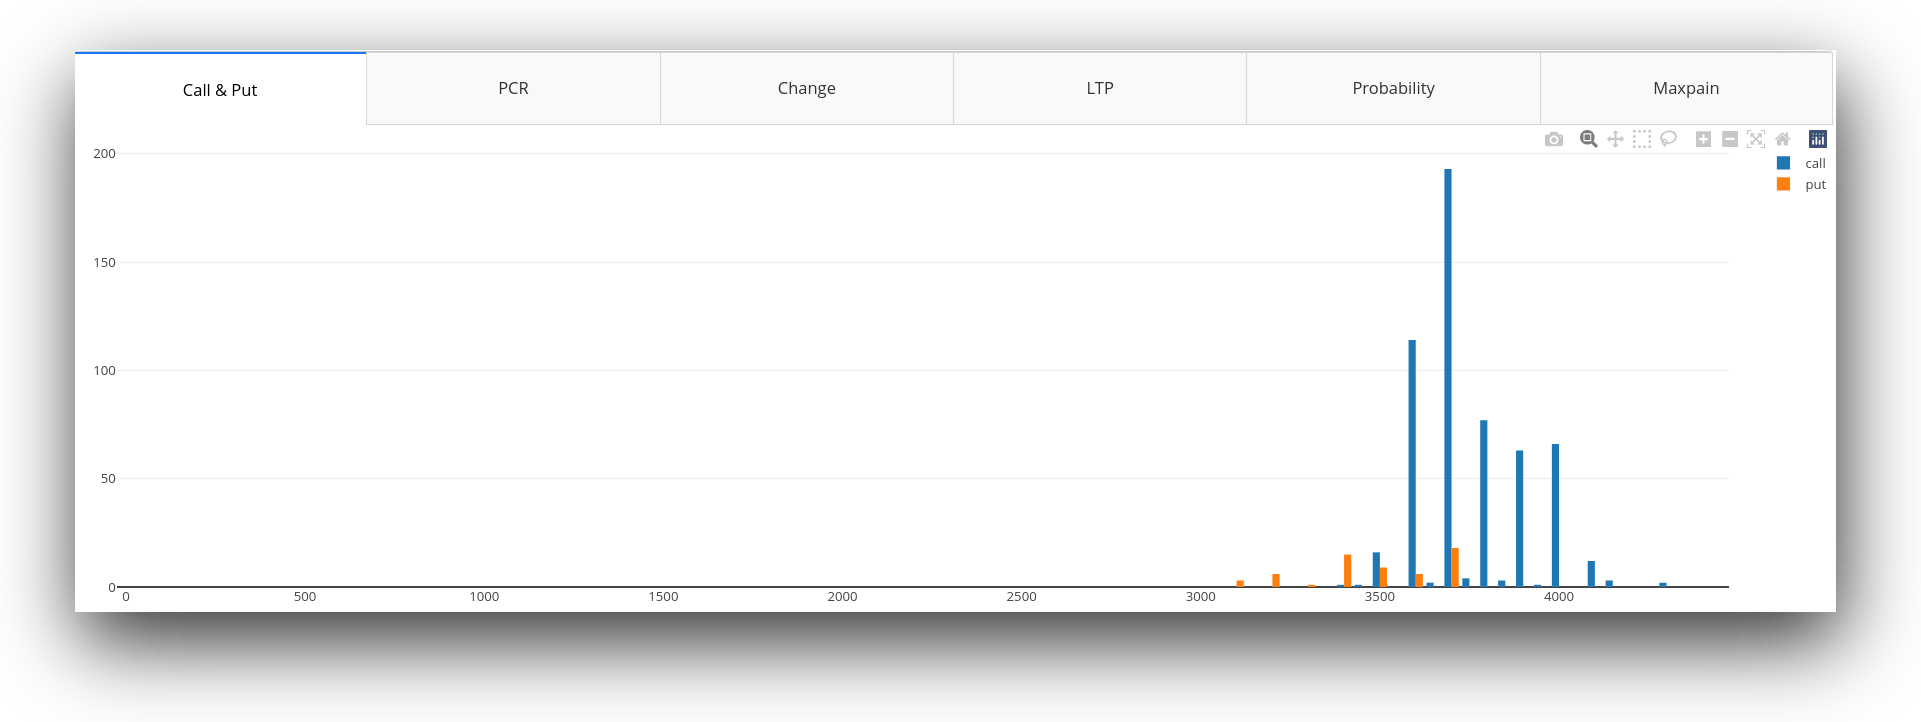
\includegraphics{calput.png}
\caption{6 tabs generated using YASP}
\end{figure}

\hypertarget{probability}{%
\subsection{Probability}\label{probability}}

\begin{figure}
\centering
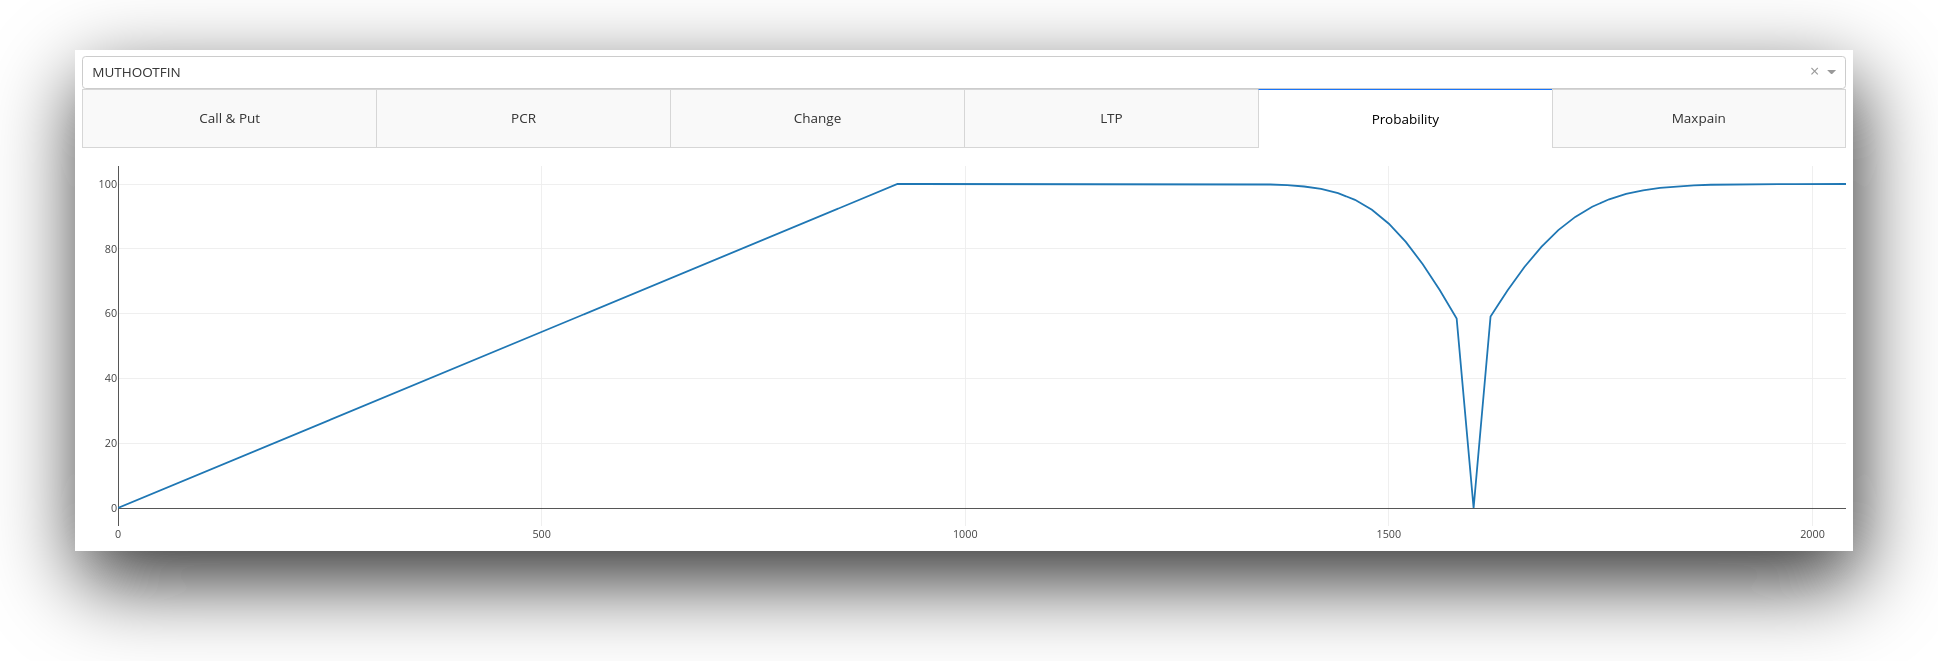
\includegraphics{prob.png}
\caption{Generated Probability Graph}
\end{figure}

\begin{multicols}{2}

\begin{itemize}
\tightlist
\item
  Left side gives the probability of stock price staying above the given
  price
\item
  Right side gives the probability of stock price staying below given
  price
\item
  At strike price probability is not calculated
\item
  Till date of expiry of contract ( option contract )
\end{itemize}

\hypertarget{maxpain}{%
\subsection{Maxpain}\label{maxpain}}

\begin{itemize}
\tightlist
\item
  Max pain, or the max pain price, is the strike price with the most
  open contract puts and calls and the price at which the stock would
  cause financial losses for the largest number of option holders at
  expiration.
\item
  The Maximum Pain theory states that an option's price will gravitate
  towards a max pain price, in some cases equal to the strike price for
  an option, that causes the maximum number of options to expire
  worthless.
\item
  Max pain calculation involves the summation of the dollar values of
  outstanding put and call options for each in-the-money strike price.
\end{itemize}

\end{multicols}

\hypertarget{scope-for-future-development}{%
\section{Scope for Future
Development}\label{scope-for-future-development}}

\begin{quote}
The investigation carried out in this work concerns graphs generated
using probability by normal distribution only. The same study can be
done by using Machine Learning (ML) methods and algorithms, namely
\textbf{LSTM}, \textbf{DRNN} and \textbf{RNN}. This may improve the data
prediction and probability of the graphs and also help in creating some
new graphs regarding future values of the stock which will be more
accurate and economic for the user.
\end{quote}

\hypertarget{references}{%
\section{References}\label{references}}

\begin{itemize}
\tightlist
\item
  https://www.investopedia.com/terms/o/optionchain.asp
\item
  https://www.investopedia.com/terms/m/maxpain.asp
\item
  https://zerodha.com/varsity/chapter/max-pain-pcr-ratio/
\item
  https://www.investopedia.com/terms/m/market-price.asp
\item
  https://www.investopedia.com/terms/s/strikeprice.asp
\item
  https://www.investopedia.com/terms/c/calloption.asp
\item
  https://www.investopedia.com/terms/p/putoption.asp
\item
  https://www.investopedia.com/ask/answers/06/putcallratio.asp
\end{itemize}
